\chapter{科技文档}

\begin{quote}
    智慧人积存知识,愚妄人的口速致败坏。
    
    \hfill《圣经·箴言》10:14
\end{quote}

现在,终于到了跟你聊聊所谓\emph{科技}文档特性的时刻。虽然关于数学式和其他方程的问题已经在第3章妥善解决,但还有一块骨头要啃:参考文献。对于这个问题,虽然不能一口吃个胖子,但接下来的内容可以让你大幅简化工作。在本章,我们还会解释生成索引的机制。

本章首先会介绍起草文章的几点特别之处,然后展示参考文献的生成和索引的生成,最后介绍将大篇幅文档拆解成几个小部分的实用方法。

\section{文章(article)}

为了起草一篇文章,没有什么新内容可以介绍的,我们目前为止见过的所有内容都适用。只需要注意,在文前部分中,可以使用以下指令:

\begin{itemize}
    \item \verb|\title|,定义标题;
    \item \verb|\date|,定义日期;
    \item \verb|\author|,定义作者团队;
    \item \verb|\thanks|,定义作者单位。
\end{itemize}

若要利用这些定义来插入标题,需要在\verb|\begin{document}|之\textbf{后}插入指令\verb|\maketitle|:

\begin{dmd}
\begin{verbatim}
\documentclass{article}
\title{Le seuillage à 128 : une révolution !}
\author{M. C. Orlanrien\\
        Institut du Pixel\\
        42007 Saint-Etienne---FRANCE}
\date{2 Avril 1927}
\begin{document}
\end{verbatim}
\backslash maketitle\textsl{\% 标题插到此处}\\
...\\
\verb|\end{document}|
\end{dmd}

此处重复一遍\jz{
    因为传授知识就是重复的过程。
}:标题是由指令\verb|\maketitle|生成并插入的,而不是文前部分的定义。

通常来说,会议或期刊提供的模板文件中会引入一些变化(例如使用\verb|\address|分隔作者和其地址),但基本原理是一致的。

\section{参考文献}

由两种方式可以使用\LaTeX 起草文章的参考文献部分。其中,可以称得上是“手动”的方式是,在文章中插入环境\dm{thebibliography}。另一种方式,即此处要介绍的方式,是使用\bib ,主要分为如下步骤。

\begin{enumerate}
    \item 创建一个或多个参数文件,包含\bib 格式的各条参考文献入口(entrée;文章、会议……)。这个步骤不可避免地需要我们去\emph{输入}。
    \item 在文档中,使用指令\verb|\cite|去引用这些入口。
    \item 参考文献会自动根据你选择的特殊风格排版。
\end{enumerate}

这种方法的优势是,对于每条参考文献,你只需输入一次。此外,考虑到可以使用\emph{风格文件},你不用去担心它的版式。有几十种风格文件,对应各种标准,包含期刊和其他会议所使用的标准。我们也可以在互联网上找到\bib 格式的参考文献数据库,可以在文档中直接使用。

我们重复一遍:参考文献有多种标准。但不幸的是,一些期刊偏偏喜欢指定属于自己的参考文献格式。有朝一日你在这种期刊上发表文章时,就需要去创建或调整风格文件。为了实现这一点,可以去查找工具\textsf{makebst}。

\subsection{\dm{.bib}文件}

第一个操作是构建\jz{
    \textbf{Emacs}的Auc\TeX 组件包含了很好用的\bib 模式。
}参考文献文件,其扩展名最好为\dm{.bib}。该文件需要遵循特殊的语法。首先需要知道,\bib 通过\emph{类型(type)}区分每个入口。这样一来,每个入口都带有一个文档类型:图书、文章、会议、科技报告……一共有二十多种不用的文档类型。

\begin{ii}
正常来说,我们可以在伴随\LaTeX 发行版提供的文件找到名为\bib ing的文件(命名为\dm{btxdoc.pdf}),由奥兰·帕塔什尼克(Oran Patashnik)在约二十年前创作。该文件包含有关构建\bib 格式文件方法的重要信息来源。
\end{ii}

每个入口\emph{类型}都包含一定数量描述该入口的\emph{字段(champ)}。参考文件入口的结构如下:

\begin{dmd}
@\codereplace{入口}\{\codereplace{关键描述},\\
\verb|  |\codereplace{字段$_1$}\ =\ \{...\},\\
\verb|  |\codereplace{字段$_2$}\ =\ \{...\},\\
\verb|  |...\\
\verb|  |\codereplace{字段$_n$}\ =\ \{...\},\\
\}
\end{dmd}

其中,\codereplace{入口}表示文档类型(\dm{article}、\dm{inproceedings}等),\codereplace{字段$_1$}、\codereplace{字段$_2$}……\codereplace{字段$_n$}表示参考文献入口的不同字段。这些\bib 的保留字可以以大写或小写形式输入。

符号\codereplace{关键描述}需要以唯一方法描述该文档,以备通过用于识别标签的符号\verb|\label|来重新找到。为了你能够快速上手\bib ,接下来的示例综合了三个你需要使用的基本入口。

\subsubsection{期刊文章}

有一篇期刊文章需要以如下形式输入:

\begin{dmd}
\begin{verbatim}
@article{qtz:UchArb,
    author ={Uchiyama, Toshio and Arbib, Michael A.},
    title = {Color Image Segmentation
            Using Competitive Learning},
    journal=pami,
    volume =16, number=2, pages={1197--1206},
    month=dec, year=1994}
\end{verbatim}
\end{dmd}

有以下几点需要注意。

\begin{enumerate}
    \item 字段\dm{author}、\dm{title}、\dm{journal}、\dm{year}是必需的。
    \item 对于作者\jz{
        此处关于作者的注意事项对于其他入口(会议、书等)也同样适用。
    }姓名,需要遵循\codereplace{姓}、\codereplace{名}的顺序。\textbf{所有}作者姓名都需要以\dm{and}分隔。
    \item 对于复合姓或其他特殊作者名,可以以如下形式输入:
    \begin{center}
        \dm{author="de la Motte Beuvron, Alain"}
    \end{center}
    其中遵循的顺序为:\codereplace{特殊组成部分}、\codereplace{姓}、\codereplace{名}。逗号作为分割符,起到与上例中相似的作用。
    \item 所有月份可以以字符串的形式给出,如\dm{jan}、\dm{feb}、\dm{mar}等。
\end{enumerate}


在\dm{.bib}文件的开头,为简洁起见,我们已经创建了\emph{缩写}\dm{pami}:

\begin{dmd}
\begin{verbatim}
@string{pami="IEEE transactions on Pattern Analysis and
              Machine Intelligence"}
\end{verbatim}
\end{dmd}

\subsubsection{会议析出文章}

没错,\bib 会区分对待\emph{期刊}和\emph{会议}中的文章。格式结构与上例很相似,只不过\dm{booktitle}用于会议标题而不是期刊标题:

\begin{dmd}
\begin{verbatim}
@Inproceedings{qtz:BouOrch,
    author={Bouman, Charles A. and Orchard, Michael T.}
    title={Color Image Display with a Limited Palette Size},
    booktitle={SPIE Conference on Visual Communications
               and Image Processing},
    volume=1199,pages={522--533},
    year=1989}
\end{verbatim}
\end{dmd}

这里,\dm{author}、\dm{title}、\dm{booktitle}、\dm{year}是必填字段,我们可以选用\dm{volume}和\dm{number}。

\subsubsection{图书片段}

相比于整本书,我们经常指参考其中的一个片段——若干章、若干页:

\begin{dmd}
\begin{verbatim}
@inBook{col:McA,
    author =    {MacAdam, David L.},
    title =     {Color Measurement},
    chapter =   4,
    pages   =   {48--49},
    publisher = {Springer-Verlag},
    year =      1985}
\end{verbatim}
\end{dmd}

强制字段为:\dm{author}、\dm{title}、\dm{chapter}或\dm{pages}、\dm{publisher} (出版方),以及\dm{year}。

\begin{ii}
我们再次强烈建议你使用Emacs组件Auc\TeX 的\textsc{Bib}\TeX 模式。特别是该模式为你提供了包含所有入口类型的菜单。选择菜单中的一项,就可以在你的文件中插入入口“骨架”。该组件可以在\wz{ftp.lip6.fr/pub/TeX/CTAN/support/auctex}下载,也可以以包Debian的形式获取。
\end{ii}

\subsection{参考文献的标注}

一旦参考文献建立完成,就可以即刻在文档中借助关键描述使用指令\verb|\cite|来标明引用:

\begin{dmd}
\backslash cite\{\codereplace{关键描述}\}
\end{dmd}

指令\verb|\cite|有如下功能:

\begin{enumerate}
    \item 根据选择的风格插入跳转符号(如[2]、[Loz95]等);
    \item 在文档的参考文献部分中添加所引用的文章。
\end{enumerate}

\begin{ii}
    文章(此处指广义的文章)只有在被\verb|cite|作为引用对象时才会出现在参考文献中。若要列出未于正文中直接引用的文章,则需要使用指令\verb|\nocite{|\codereplace{关键描述}\verb|}|将\codereplace{关键描述}的对应文章插入文档的参考文献部分。此外,指令\verb|\nocite{*}|会将\dm{.bib}文件中的\emph{所有}入口插入文档。
\end{ii}

在实际进入生成参考文献的步骤前,需要在\LaTeX 文档末尾添加对以下指令的引用来指定参考文献的风格:

\begin{dmd}
\verb|\bibliographystyle|
\end{dmd}

然后,引用如下指令来实际插入参考文献:

\begin{dmd}
\verb|\bibliography|
\end{dmd}

对于风格,有:

\begin{dmd}
\backslash bibliographystyle\{\codereplace{风格}\}
\end{dmd}

\LaTeX 预定义的风格\jz{
    在CTAN网站的\dm{biblio/bibtex/contrib}可以找到几十种可供使用的其他风格。
}如下。

\begin{itemize}
    \item \dm{plain},引用的形式为[2],参考文献会根据作者名排序。
    \item \dm{unsrt},参考文献根据引用顺序排序。会议文章经常使用这种风格。
    \item \dm{alphs},引用的形式为“作者缩写+年份”。
\end{itemize}

接下来,需要指定哪些文件包含了文档中指令\verb|\cite|所“指向”的那些参考文献:

\begin{dmd}
\backslash bibliography\{\codereplace{文件$_1$}, \codereplace{文件$_2$}, \codereplace{……}\}
\end{dmd}

这样的指令会使\bib 在处理过程中包含\codereplace{文件$_1$}\dm{.bib}、\codereplace{文件$_2$}\dm{.bib}……

\subsection{生成参考文献}

生成参考文献的步骤如下。

\begin{enumerate}
    \item 借助\LaTeX 实现第一次编译,使得辅助文件\dm{doc.aux}包含\emph{引用标注}信息:
    
    \begin{center}
        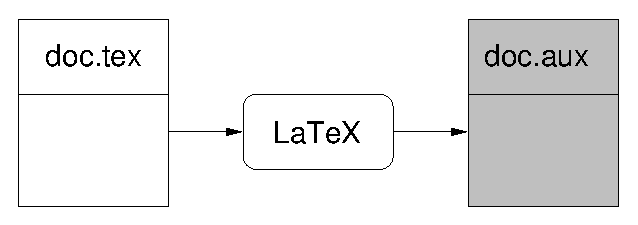
\includegraphics{img/bibtex1}
    \end{center}
    
    \item 运行\bib ,在文件\dm{doc.bbl}中生成参考文献:
    
    \dmh{bibtex doc}

    \begin{center}
        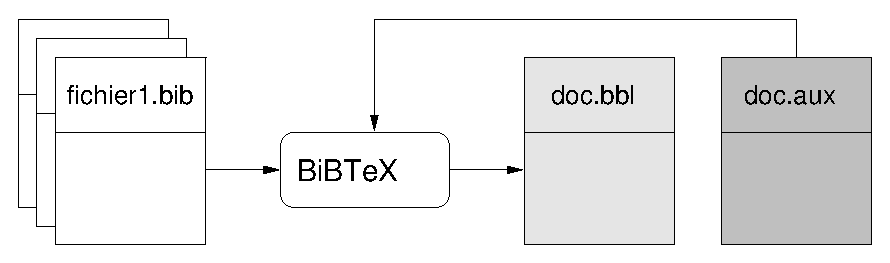
\includegraphics{img/bibtex2}
    \end{center}

    \item 借助\LaTeX 的第二次编译插入参考文献:
    
    \begin{center}
        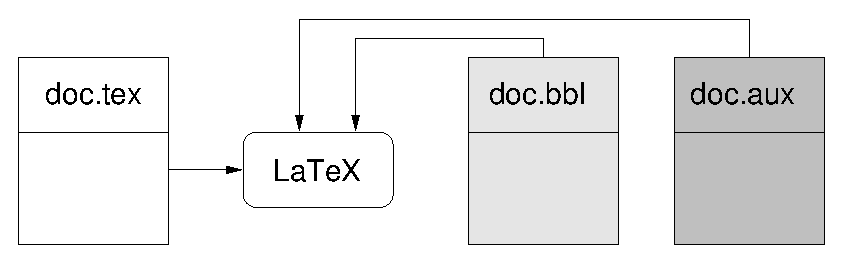
\includegraphics{img/bibtex3}
    \end{center}

    %TODO 图片中bibtex和latex替换

    \item 通过第三次编译解析交叉引用。
\end{enumerate}

如果你对这个过程感到好奇,可以看到:文件\dm{doc.bbl}包含了环境\dm{thebibliography}以供随时使用\jz{
    也就是说,你如果不使用\bib ,就必须着手处理该环境。
};文件\dm{doc.blg}是与那些\dm{.log}文件相似的“日志”文件,储存着上一次使用\bib 时一些可能出现的错误或警告。

\begin{exclamation}
程序\bib 对环境\dm{BIBINPUTS}中的参数敏感。因此,在某些情况下,有必要在\linebreak\dm{.bash\_profile}中添加以下一行命令:

\dmh{export BIBINPUTS=\$HOME/LaTeX/biblio//:}

这样可以使\bib 在目录\dm{\$HOME/LaTeX/biblio}中搜索你的参考文献文件(此处的目录为示例)。
\end{exclamation}

\section{索引}

生成索引需要依靠以下两个概念:

\begin{enumerate}
    \item 在\LaTeX 文档中添加指令\verb|\index|来添加索引入口;
    \item 使用程序\textbf{makeindex}来正确地抽取和展示索引。
\end{enumerate}

负责在文档中插入索引部分的是指令\verb|\printindex|。可以将该指令与\verb|\tableofcontents|类比。

\subsection{必要步骤}

这里给出简短的索引制作备忘录:

\begin{enumerate}
    \item 在主文件中插入两条指令:
    \begin{dmd}
    \begin{tabbing}
12345678902234567890\=\kill
\verb|\makeindex|\>\textsf{$\leftarrow$告知\LaTeX 需要生成索引}\\
\verb|\begin{document}|\\
{\rmfamily ……文档正文……}\\
\verb|\printindex|\>\textsf{$\leftarrow$在文档中实际插入索引部分}\\
\verb|\end{document}|
    \end{tabbing}
    \end{dmd}

    \item 插入索引入口:
\begin{dmd}
\begin{tabbing}
12345678902234567890\=\kill
\verb|\index{bidule}|\>\textsf{$\leftarrow$在索引中插入“bidule”}
\end{tabbing}
\end{dmd}

    \item 为了为文档\dm{doc.tex}生成索引,需要成功执行以下三条指令:
    
    \begin{dmd}
        latex doc\\makeindex doc\\latex doc
    \end{dmd}
\end{enumerate}

\subsection{机制细节}

文档\dm{doc.tex}的第一次编译(在满足文前部分带有控制序列\verb|\makeindex|的条件下)会生成包含“散装”的索引入口文件\dm{doc.idx}:

\begin{center}
    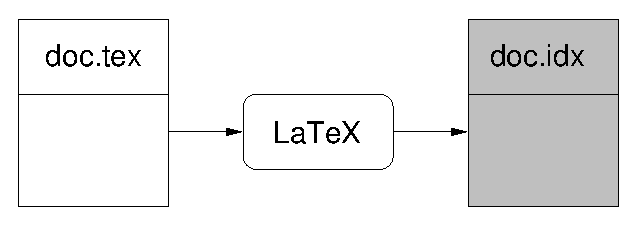
\includegraphics{img/makeindex1}
\end{center}

接下来,使用\textsf{makeindex},在这个文件\dm{doc.idx}中整理条目、删除重复项,并将结果存入\dm{doc.ind}。执行轨迹会存储在\dm{doc.ilg}中:

\begin{center}
    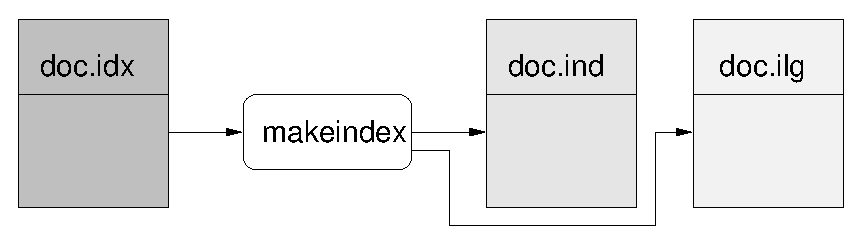
\includegraphics{img/makeindex2}
\end{center}

终端下运行的\textsf{makeindex}嘴很碎。如下展示了它生成文档索引时展示的信息:

\begin{dmd}
\begin{verbatim}
This is makeindex, version 2.13 [07-Mar-1997] (using kpathsea).
Scanning input file guide.idx....done (982 entries accepted, 0 rejected).
Sorting entries...........done (11254 comparisons).
Generating output file guide.ind....done (745 lines written, 0 warnings).
Output written in guide.ind.
Transcript written in guide.ilg.
\end{verbatim}
\end{dmd}

因此,在运行失败的情况下,需要警惕可能出现的抛出和警告(\emph{warning})。\LaTeX 的第二次编译可以在\dm{doc.tex}中指令\verb|\printindex|指出的位置插入格式化过的索引(文件\dm{doc.ind}):

\begin{center}
    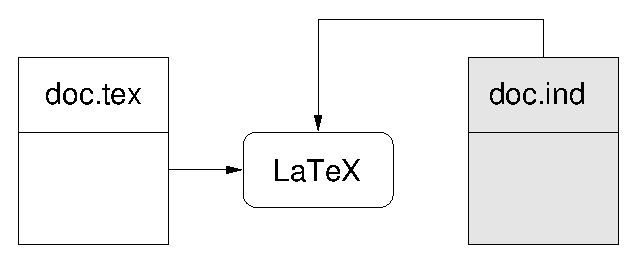
\includegraphics{img/makeindex3}
\end{center}

\begin{ii}
工具makeindex可以识别选项\dm{-s},该选项用于为索引指定\emph{风格}。这里所说的风格定义在带有扩展名\dm{.ist}的文件中,可以改变索引的排版央视。可以以如下方式修改文件风格:

\dmh{makeindex -s}\codereplace{文件风格}\codereplace{主文件}

可以在你使用的发行版中寻找风格文件并测试它们。
\end{ii}

\subsection{索引入口的不同类型}

目前为止,我们看到的索引形式都是\emph{\codereplace{索引词}及\codereplace{页码}},但也可以使用更讲究些的入口形式,至少包含如下三种。

\begin{enumerate}
    \item 带有层级的入口:
    
    \begin{dmd}
    \verb|\index{bidule!chouette}|
    \end{dmd}

    该指令可以在索引中插入“bidule”的子入口“bidule”。

    \item 跨页入口:
\begin{dmd}
\begin{tabbing}
12345678902234567890\=\kill
\verb+\index{bidule|(}+\>\textsf{$\leftarrow$位于第$i$页}\\
\verb+\index{bidule|)}+\>\textsf{$\leftarrow$位于第$j$页}
\end{tabbing}
\end{dmd}
    该指令插入的索引形式为bidule $i$--$j$。

    \item 符号化的入口:
    
    \begin{dmd}
    \verb|\index{alpha@\alpha}|
    \end{dmd}

    这样的指令会在索引中插入$\alpha$,并按“alpha”将其分类。同样地,以下指令会在索引中插入“épluche”,但分类时会将首字母看作“e”:

    \begin{dmd}
    \verb|\index{eplucher@éplucher}|
    \end{dmd}
\end{enumerate}

此处列出的最后一个格式同样可以用于为索引插入带有特殊版式的入口。例如:

\begin{dmd}
\verb|\index{bonjour@\textbf{bonjour}}|
\end{dmd}

该指令可以在索引中插入\textbf{bonjour}(即将bonjour加粗),同时按“bonjour”将该入口分类。此外,借助以下指令,我们还可以以特殊版式显示页码:

\begin{dmd}
\backslash index\{\codereplace{入口}|\codereplace{版式指令}\}
\end{dmd}

例如:

\begin{dmd}
\verb+\index{bidule|textbf}+
\end{dmd}

该指令可以让索引中“bidule”的页码显示为加粗样式(注意,在版式指令中没有符号\verb|\|)。

\subsection{术语词典}

有时,我们需要详细列出文档中一些术语的含义。文档中重新组织这些术语解释的部分称为\emph{术语词典(glossaire)}。为了生成术语词典,需要采用与生成\celan{\S 6.3.1}索引相似的方法,只需做一些小的改动,将在11.6节详细介绍。

\section{拆分文档}

如果文档的篇幅很长,我们可以将其自然地按章或部分来拆解。因此,建议创建一个\emph{主}文档,并在其中包含各章或各部分。主文档的形式如下:

\begin{dmd}
\begin{verbatim}
\documentclass{book}

\begin{document}
\end{verbatim}
\verb+\frontmatter +\textsl{\% 所有介绍性的文字}
\begin{verbatim}
\include{preface}
\tableofcontents
\end{verbatim}
\verb+\mainmatter +\textsl{\% 文档的“主体”}
\begin{verbatim}
\part{关于\LaTeX 的那些你想知道却从不敢问的问题}

\chapter{基本原则}
\begin{quote}
    人若身患漏症,他因这漏症就不洁净了。——《圣经·利未记》15:2
\end{quote}

本章介绍\LaTeX 的基本原理。你将会看到关于\LaTeX 安装的简介、使用\LaTeX 的基本“流程”(session)介绍、文章格式的结构、使用变音符号的注意事项,认识几个工具,以及了解面对编译错误消息时的态度。

\section{安装}

你想安装\LaTeX 吗?你将要安装的是\LaTeX 的其中一个\textit{发行版},具体的版本取决于你的操作系统\jz{
    如果你不知道操作系统是什么东西,那么你使用的是macOS;如果你不知道你的计算机用的\textit{具体是哪个}操作系统,那么你在用Windows;否则,你在用UNIX……
}。发行版中带有可以自动安装和配置\LaTeX 、\TeX 和其他相关内容的程序。

\paragraph*{对于UNIX}我们可以找到称为te\TeX 的发行版,虽然它的开发早在2006年就停止了。今天,我们一般安装\TeX Live(\wz{http://www.tug.org/texlive})。

\paragraph*{对于macOS}建议安装的发行版是Mac\TeX(\wz{http://www.tug.org/mactex})。

\paragraph*{对于Windows}最简单的方式无疑是选择pro\TeX t(\wz{http://www.tug.org/protext})。它会安装称为MiK\TeX 的发行版(\wz{http://www.miktex.org})和几个开发工具,其中包含一个查看PostScript文件的程序(\textsf{gsview})。

偶尔,需要在为发行版中搭配一款文字编辑器(如果其中没有包含),因为你很快就能看到,使用\LaTeX 就是在文件中输入文字和命令。

\begin{itemize}
    \item UNIX中,推荐使用\textsf{emacs}或\textsf{vi},即使前者明显比后者更高级,但二者用户之间无结果的恶意争吵仍在继续。
    \item \textsf{kile}和\textsf{texmaker}是已集成的开发环境。依靠它们,初学的用户在入门时会觉得更轻松。它们的特点是将编辑、编译和可视化集成在一个界面。这两个环境也使通过菜单、对话框或其他标签来探索\LaTeX 指令称为可能(如图\ref{fig:1.1}a所示)。
    \item Windows中的对应产品是\textsf{\TeX nicCenter}(如图\ref{fig:1.1}b所示)。
    \item macOS中的对应产品是\textsf{\TeX shop}和\textsf{i\TeX max}。
\end{itemize}

\begin{figure}%[H]
    %TODO 图
    \centering
    \includegraphics[width = 0.8\linewidth]{img/kile.eps}\\
    (a) Kile\\
    \includegraphics[width = 0.8\linewidth]{img/texniccenter.eps}\\
    (b) \TeX nicCenter
    \caption{集成的两个开发环境:Linux中的Kile和Windows中的\TeX nicCenter。它们将编辑、编译和可视化集成在一个界面中}
    \label{fig:1.1}
\end{figure}

你很快就会学到,用\LaTeX 制作文档是一个翻译(也称作\textit{编译})的过程——将编辑者创建的源文件转换为用于显示或印刷的格式\jz{本章会略微多介绍一些这个格式。}。因此,发行版中内置了或多或少的著名工具,可以将编译后的不同格式的文件显示出来。

\paragraph*{对于PDF格式}除了著名的\textsf{acrobat reader},UNIX中还有一些可以显示PDF文件,如\textsf{xpdf}、\textsf{evince}等。

\paragraph*{对于DVI格式}UNIX中的\textsf{xdvi}、\textsf{kdvi}和Windows中的\textsf{yap}都是可以显示这种\LaTeX 编译文件的程序。

\paragraph*{对于PostScript格式}\textsf{ghostscript}套件(在各平台下的名称可能有差异)可以显示PostScript文件。

\begin{exclamation}
    需要注意,为了使你选用的发行版包含\LaTeX 的“法文”模式,以确保能够正确处理断字(césure;英:hyphenation),我们需要在编译文档是需要更改其“日志”(见1.6节)%带有引用
    以使法文模式加载:

    \begin{dmd}
    LaTeX2e <2005/12/01>\\
    Babel <v3.8h> and hyphenation patterns for english, [...] dumylang, \fbox{french}, loaded.
    \end{dmd}
\end{exclamation}

\section{“生产”周期}

即使\LaTeX 并不是通常意义上说的编译型语言,但我们仍然可以将制作一个\LaTeX 文档的周期与使用一款经典的编程语言开发软件的\textit{编辑—编译—执行}周期进行类比。

\subsection{编辑}

一个\LaTeX \textit{源}文件是一个文本文件\jz{即文件仅由组成其中符号的代码构成。}。因此,对\LaTeX 文件的操作并不依赖于某个特定的软件,只需要一个经典的文本编辑器即可。因此,若要操作\LaTeX 文档,指令

\dmh{emacs \codereplace{文件名}.tex \&} %TODO <>

或

\dmh{vi \codereplace{文件名}.tex}

足以让你进入\LaTeX 文档这个充满野性和未知的世界。在Windows中,根据自己的喜好,我们可以选用一款文字编辑器。注意,对于\LaTeX 源文件,推荐使用\dm{.tex}扩展名名。

\subsection{编译}

我们用如下指令开始编译:

\dmh{pdflatex \codereplace{文件名}.tex}

早晚有一天,你会看到编译会产出错误。这将是1.6节会处理的问题。总之,解决了编译问题后,我们会得到一个带有\dm{.pdf}扩展名的文件,它代表\textit{便携文件格式(英:portable document format)},这是一种由Adobe公司创造的著名格式。

\begin{ii}
    历史上,编译\LaTeX 源文件会生成\dm{dvi}文件,代表\textit{设备无关(英:device independant)}。此类文件独不受输出环境(如屏幕、打印机等)的影响。这是一种包含了“图像”的\LaTeX 便携二进制文件,可以用于各种操作系统。随后,出现了一批用途各异的程序:
    \begin{itemize}
        \item 用于显示文档,即\dm{.dvi}\rightarrow 点阵屏幕;
        \item 用于打印,即\dm{.dvi}\rightarrow 打印机语言;
        \item 用于转换格式,即\dm{.dvi}\rightarrow PostScript文件。
    \end{itemize}
\end{ii}

图\ref{fig:1.2}表明了UNIX生成最终文件过程中参与流程的多种程序。

\begin{ii}
    除了使用pdflatex外,也可以使用其他“编译器”来生成PDF文件。例如,xelatex和lualatex可以能正确地处理以UTF-8编码的文件,是常用的替代选项。
\end{ii}

\begin{figure}[H]
    %TODO 图
    \centering
    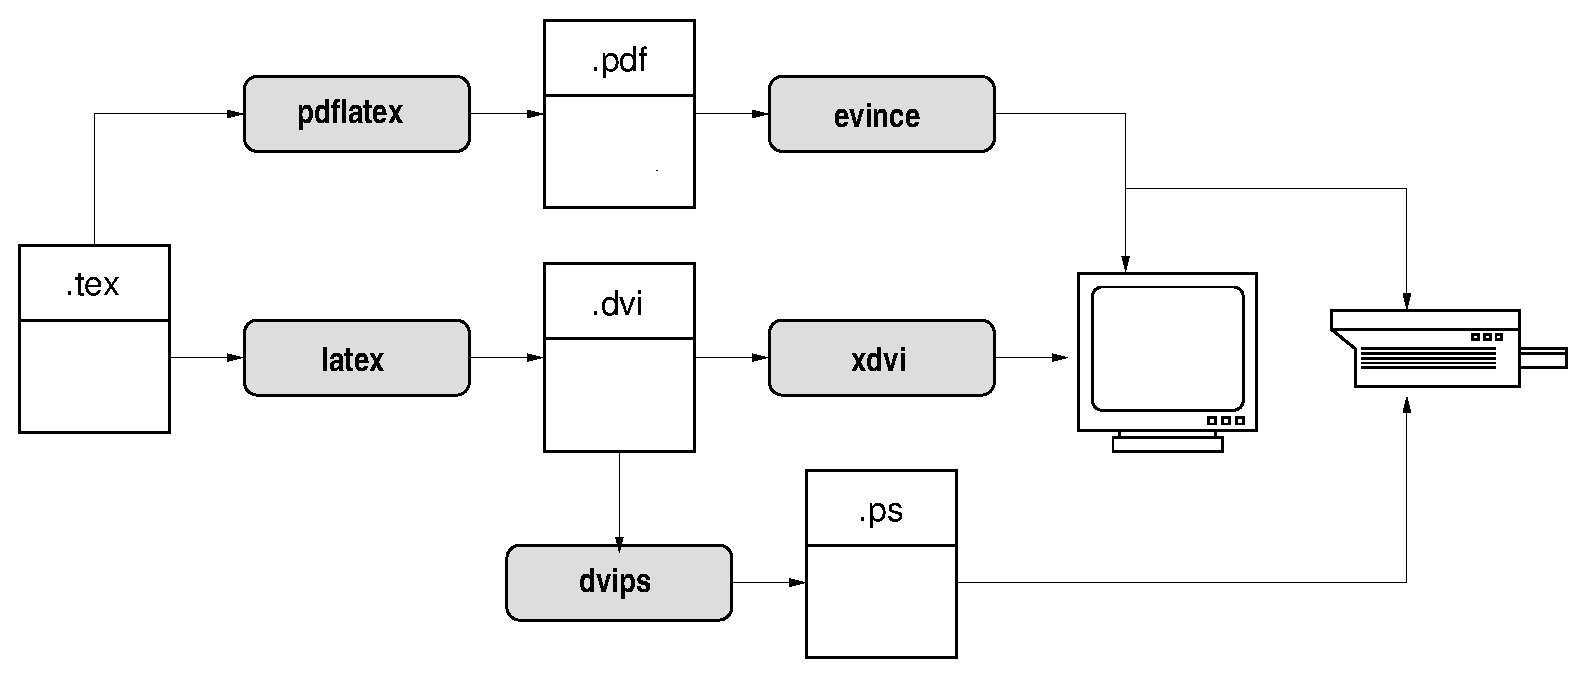
\includegraphics[width = 0.8\linewidth]{img/cycle.eps}
    \caption{UNIX中参与生成过程的工具}
    \label{fig:1.2}
\end{figure}

\subsection{显示}%visualisation有时翻译成可视化,有时翻译成显示,这个可以后期再统一一下。

在编译后,可以简单地使用\textsf{evince}程序来完成显示步骤。输入以下指令:

\dmh{evince \codereplace{文件名}.pdf \&}

这是一个\textsf{linux}下运行的十分直观的程序,能够给出一个方便阅读的文件预览。

\begin{exclamation}
    注意,不必在每次编译后都重新运行evince,它显示的内容会自动刷新。
\end{exclamation}

\subsection{打印}

对于\dm{pdf}格式,如何打印它这一问题就丢给了你的操作系统。关于这一点,没有特殊的注意事项。你有了一个文件,可以自由地处置它,无论是直接打印,还是根据你所处的环境来发挥才艺。

\begin{ii}
    从\dm{dvi}到\dm{ps}格式的转换需要调用dvips程序:

    \dmh{dvips \codereplace{文件名}.dvi}

    这可以生成一个PostScrpt格式的文件。这个格式也由Adobe创造,是一种打印机语言,可以看作\dm{pdf}的祖先。目前的打印机出厂即可识别这种打印机语言。我们可以说,文件发送到打印机时,十有八九传送的是PostScrpt格式的参数。对于PostScript格式的文件,有大量可以显示、修改这种文件的工具。
\end{ii}

\section{源文件的结构}

本节将介绍一种文档类型。实际上,所有\LaTeX 文档都具有相同的结构,形式如下:

\begin{dmd}
\backslash documentclass[\codereplace{类选项$_1$},\codereplace{类选项$_2$},...]\{\codereplace{类}\}\\
\backslash usepackage[\codereplace{包选项$_1$},\codereplace{包选项$_2$},...]\{\codereplace{包}\}\\
...\\
\codereplace{文前部分}\\
...\\
\backslash begin\{document\}\\
...\\
\codereplace{文本}\\
...\\
\backslash end\{document\}
\end{dmd}

如此一来,所有的\LaTeX 文档都可以按以下方式拆解。

\begin{itemize}
    \item 说明文档的\codereplace{类};
    \item 文前部分,包含以下内容:
        \begin{itemize}
            \item 使用特定的\codereplace{包};
            \item 多样的初始化和声明;
        \end{itemize}
    \item 文档主体,即我们将要亲手输入的全部内容,出现在\dm{\backslash begin\{document\}}和\dm{\backslash end\{document\}}之间。
\end{itemize}

以下介绍各部分的细节。

\subsection{文档的类}

所谓类,就是提供给\LaTeX 的一个指示,可以帮助\LaTeX 决定如何为文档的特定部分排版。根据具体使用的类不同,允许使用与否的指令可能不同(如\dm{\backslash chapter}在\dm{book}类中允许使用,在\dm{article}类中不允许使用)。另一方面,根据所选择的类,给出的命令会具有特定的含义(标题、材料表……)。在入门时\jz{
    实际上,我们可以在\dm{\backslash documentclass}前添加更多神奇的“咒语”……
},所有的\LaTeX 文档都必须以的指令开始——\dm{\backslash documentclass}接由花括号括住的类,包含以下几种:

\begin{itemize}
    \item \dm{article},用于文章;
    \item \dm{proc},用于电气与电子工程师协会(英:Institute of Electrical and Electronics Engineers,IEEE)会刊(英:proceeding)风格的文章;
    \item \dm{report},用于几十页篇幅的报告;
    \item \dm{book},用于图书或论文;
    \item \dm{letter},用于信件;
    \item \dm{slides},用于演示文档。
\end{itemize}

我们当然也可以为文档定义自己的类。类的配置项用方括号括住,可以是以下内容之一:

\begin{itemize}
    \item \dm{11pt, 12pt},用于全局地更改文字字号;
    \item \dm{twoside},用于生成适合双面打印的文档;
    \item \dm{draft},用于以草稿模式生成文档。
\end{itemize}

例如,输入:

\begin{dmd}
\verb|\documentclass{article}|
\end{dmd}

以上命令可以将全部配置项配置为默认值(字号为10 pt,单列,单面……)。

\begin{dmd}
    \backslash documentclass[12pt]\{article\}
\end{dmd}

以上命令将字号设置为12 pt(默认为10 pt)。再如:

\begin{dmd}
    \backslash documentclass[twoside, draft]\{report\}
\end{dmd}

以上命令可以以草稿模式生成适合双面打印的报告。

\subsection{文前部分}

文前部分是指位于子句\dm{\backslash documentclass}和子句\dm{\backslash begin\{documennt\}}间的区域。在这个区域中,我们可以明确想要包含的扩展(请看下一小节)%TODO
、初始化全局参数(如页边距等)、定义风格(如标题样式、序号等)、定义特殊的宏,等等。

\subsection{添加扩展}

\LaTeX 命令\dm{\backslash usepackage}可以与C语言的指令\dm{\#include}类比。这一命令允许添加\LaTeX 中满足宏或环境形式的功能\jz{
    相关内容将在下一章讲解。%TODO
}。目前,只需记住,我们可以在一行之内包含多个包:

\begin{dmd}
    \backslash usepackage\{\codereplace{包$_1$},\codereplace{包$_2$},\codereplace{包$_3$},...\}
\end{dmd}

如果\codereplace{包$_1$}、\codereplace{包$_2$}、\codereplace{包$_3$}拥有共同的配置项\codereplace{opt1},我们可以输入:

\begin{dmd}
    \backslash usepackage[\codereplace{opt1}]\{\codereplace{包$_1$},\codereplace{包$_2$},\codereplace{包$_3$}\}
\end{dmd}

相反,如果\codereplace{opt1}只涉及\codereplace{包$_2$},那么我们只能像这样写成两行:

\begin{dmd}
    \backslash usepackage\{\codereplace{包$_1$},\codereplace{包$_3$}\}\\
    \backslash usepackage[\codereplace{opt1}]\{\codereplace{包$_2$}\}
\end{dmd}

下面是两个例子:

\begin{dmd}
    \% 包graphicx带有配置项draft和xdvi\\
    \backslash usepackage[xdvi, draft]\{graphicx\}\\
    \% 包array和包subfig\\
    \backslash usepackage\{array, subfig\}
\end{dmd}

\begin{exclamation}
    根据定义,所有(类、包、命令的)的配置项参数都是\textit{可选的}。因此我们可以这样记:\LaTeX 中所有由方括号括住的参数\dm{[...]}都是非强制的。
\end{exclamation}

\section{开始!}

在本节,我们将尝试从一个只含几个排版命令的文档开始,介绍\LaTeX 的基本原理。

\begin{codelist}[1.1]{
    从你手中掉落的工具总是掉到最难够到的地方,或脆弱的物品上。\\
    这是\emph{墨菲}定律(loi de Murphy)的一个体现。
}  \begin{dmd}
    \verb+\documentclass{article}+\\
    \verb+\begin{document}+\\
    从你手中掉落的工具\\
    总是掉到最难够到的地方,\\
    或脆弱的物品上。\\
    ~\\
    \verb+这是\emph{墨菲}定律(loi de      Murphy)的+\\
    一个体现。\\
    \verb+\end{document}+
\end{dmd}
\end{codelist}

这个示例体现了\LaTeX 中的几个重要的原理,具体如下。

\paragraph*{空行代表跳转至下一段} \LaTeX 中的空行代表一段文字的结尾,因此在以上实例中,第一段从“\dm{从你}”开始,直到“\dm{物品上。}”结束。指令\dm{\backslash par}与空行等价,可以用来表示一段文字的起始。

\paragraph*{\LaTeX 会忽略换行}最终的文档中,换行并不由源文件中的换行决定。\LaTeX 会自动为各段文本\textit{打断、压缩、调节}文字,除非你有特殊的要求。

\paragraph*{\LaTeX 会忽略重复的空格}输入1个或18784个空格是等价的,比如源码中\dm{de}和\dm{Murphy}前插入的空格那样。此规则也适用于跳转段落:输入一行或多行空格是等价的。

\paragraph*{“\backslash ”是转义字符(caractère d’échappement;英:escape char)}“\backslash ”可以告诉\LaTeX 它后面的一系列字符是控制序列,也就是说,是最一般意义上的指令(或宏)。这里,它对“墨菲”一词生效,具体的效果由指令\dm{\backslash emph}控制。

\paragraph*{“\{”和“\}”}它们是\textit{组}的定界符,稍后会进一步解释它们。

\subsection{几个特殊字符}

就像符号“\backslash”的出现所暗示的那样,\LaTeX 中还有10个有特殊含义的符号,在此将其列出:

\begin{dmd}
    \verb+\ $ & % # ^ _ { } ~+
\end{dmd}

%todo 此前代码可以重新简化为verb

以下是一个使用部分特殊字符的案例:

\begin{codelist}[1.2]{
\textbf{是}下标:$x_{i+1}$,还是上标:$e^{i\pi}$;这是问题~1!
}\begin{verbatim}%毫无意义的段落
\textbf{是}下标:$x_{i+1}$,
还是上标:$e^{i\pi}$;
这是问题~1!%还是问题2?\end{verbatim}
\end{codelist}

目前,你需要知道:

\begin{itemize}
    \item \dm{\%}会使得\LaTeX 忽略当前行的剩余部分,因此,它是表示注释的符号(与C中的\dm{//}等价);
    \item \verb+~+代表不可拆分的空格\jz{
        见2.10节。
    },可以防止\LaTeX 在指定的位置断字。尽管有大量的情况需要插入这个符号来表示不可拆分(如所有形如“\verb+图~1+”的情况),然而,对于此类符号的使用,并没有系统化的规则。
    \item \dm{\$}用于标记公式的开始和结束。\LaTeX 遇到一个\dm{\$}符号时,它会切换到\celan{第3章}数学模式,直到遇到下一个\dm{\$}符号。
    \item \dm{\_}和\dm{\^{}}分别代表将文本转化为下标和上标。\textbf{注意},这两个符号只能在数学模式下使用。
    \item \dm{\{}和\dm{\}}分别表示组的开始和结束。本例中出现了两种组:一种出现在数学模式中,用于把将要放到下标或上标的“子公式”组合起来;另一种把将要设置成粗体的文字组合起来。
\end{itemize}

我们可以使用如下的指令来在让文档生成部分特殊字符:

\begin{dmd}
    \verb+\$ \& \% \# \{ \} \_+
\end{dmd}

这串指令可以输出“\$ \& \% \# \{ \} \_”。2.2.5小节%TODO
会解释如何使文档生成其余特殊字符(即\verb+\ ~ ^+)。

\subsection{调用指令}

你已经知道了,要想调用指令或宏,需要输入转义字符,并紧接着输入你想使用的宏名。%TODO 二对一
但是,\LaTeX 如何知道宏名的末尾在哪里呢?此处以用于生成\TeX 标识的\dm{\backslash TeX}为例来解释\yz{
    此例涉及对西文行文中空格的处理,不宜翻译。
}。

\begin{codelist}{
    \TeX book is for \TeX hackers.

    \TeX\  has some powerful macros.

    \LaTeX{} is a document preparation system
}\begin{verbatim}\TeX book is for \TeX hackers.

\TeX\  has some powerful macros.

\LaTeX{} is a document preparation system
    \end{verbatim}
\end{codelist}

\begin{exclamation}
    \verb*|\ |(其中\verb*| |代表空格)称作控制空格(espace de contrôle)。这个空格不会被\LaTeX 忽略。因此,指令“\verb*|et\ \ \ hop !|”会生成“et\ \ \ hop !”。实际上,以\dm{\backslash}\codereplace{函数}\dm{\{}\codereplace{参数}\dm{\}}的形式来调用宏是很好的习惯。因此,使用上例中的的第三种方式比第二种方式更佳。这种形式可以避免空格被忽略的情况发生\jz{
        所以他为什么要跟我们说这些?!
    }。因此,我们将使用\verb|the \teX{}book|来生成“the \TeX{}book”,使用“\verb*|\LaTeX{} is a ...|”来生成“\LaTeX{} is a ...”。
\end{exclamation}

\subsection{变音符号}

法国人往往对于使用\LaTeX 这件事忧心忡忡,因为法文中带有变音符号。别怕!你不必像表\ref{tab:1.1}\yz{
    该表与原书不完全相同。
}中展示的那样输入带有变音符号的字符。然而,你需要知道:无论是什么种类的字符,包括大写字母,我们都可以为其添加变音符号。

\begin{table}[H]
    \centering
    \begin{tabular}{|c|c|c|}
        \hline
        变音符号 & 源码 & 效果\\
        \hline
        尖音符 & \verb|\`z| & \`z \\
        钝音符 & \verb|\'z| & \'z \\
        长音符 & \verb|\^z| & \^z \\
        软音符 & \verb|\c{z}| & \c{z}\\
        分音符 & \verb|\"{z}| & \"{z}\\
        \hline
    \end{tabular}
    \caption{输入占7位(bit)的变音符号}
    \label{tab:1.1}
\end{table}

注意!虽然我们可以输入带有变音符号的字符,但不要忘记:这需要我们调用编码。目前,编码可能只针对地球上的某个地区。在法国,我们使用ISO 8859编码,配合拉丁文1区拓展。这套编码允许我们操纵美丽的变音符号。在详细阅读本书中专为使用法文书写文档的情况准备的章节\celan{第7章}之前,我们建议你在你源码的文前部分添加以下指令,以“攻克”法文文档的难关:

\begin{dmd}
    \begin{verbatim}
%源文件编码
\usepackage[latin1]{inputenc}
%TeX字体编码
\usepackage[T1]{fontenc}
%针对法文文档
\usepackage[francais]{babel}
    \end{verbatim}
\end{dmd}

\section{第一批工具}

以下几个宏和合字在文档中很常用,因此应当了解它们。首先,\LaTeX 会区分三种连接号:

\begin{itemize}
    \item \verb|-|,用于“Saint-Étienne”;
    \item \verb|--|,用于“page 12--24”;
    \item \verb|---|,在法文中用于插入语,如“une parenthèse --- comme cela”。
\end{itemize}

引号应以如下方式输入:

\begin{itemize}
    \item \verb|``|和\verb|''|可以输入英文中的引号\yz{
        此处与原书不同。原书前文输入变音符号时亦直接使用了单弯引号‘和’,但这两个符号作为命令参数时会导致编译错误,因此分别替换为反引号和直单引号。这可能是编译器的差异导致的。
    }——``English''。
    \item 如果键盘允许,对于法文,你可以输入«和»\jz{
        例如,在Linux系统下,分别按键盘的\fbox{Alt Gr}+\fbox{Z}和\fbox{Alt Gr}+\fbox{X}组合键(译注:适用于AZERTY键盘)。
    }。\textsf{babel}包的法文支持部分(参考第7章)%TODO
    允许我们通过\verb|\og|和\verb|fg|输入引号,由此,\verb|\og français\fg{}|这类命令是允许的—— «~français~»~。
\end{itemize}

以下是其余几个使用的命令:

\begin{itemize}
    \item \verb|\today|可以生成(编译时的)日期——2013年11月22日。
    \item \verb|\S|可以生成段落符号——\S。
    \item \verb|\ldots|可以在英文文档中生成省略号“\ldots”。但在法文文档中,应当输入三个点“...”(第7章会介绍更多有关法文排版的内容)。%TODO
\end{itemize}

最后要记得,英文中的双成分标点(ponctuation double;包括:;!?)前不加空格,但法文相反,它们的前面需要加空格。另外,在法国这个可爱的国家,我们几乎都靠右行驶。

\section{第一组报错}

\begin{ii}
    接下来,我们会看看\LaTeX 编译你的文档时闹的“情绪”。当我们放出编译指令时,我们会直接在终端看到这些输出。为了能让\LaTeX 得到充分使用,我们鼓励你在自己的环境下找到属于你自己的检查\LaTeX “\textsf{日志}”的方法。这些日体可以为你指明错误信息,以及编译过程中出现的其他警告。
\end{ii}

\subsection{症状}

如果你与\LaTeX 打交道,那么早晚有一天,你会看到屏幕上显示出类似这样粗旷的信息:

\begin{dmd}
    \linenumbers
    \begin{verbatim}
This is TeX, Version 3.1415 (C version 6.1)
(erreur.tex
LaTeX2e <1995/12/01>
(/usr/local/lib/texmf/tex/cls/article.cls
Document Class: article 1995/11/30 v1.3p Standard LaTeX document class
(/usr/local/lib/texmf/tex/clo/size10.clo)) (erreur.aux)
! Undefined control sequence.
l.5 paragraphe de ce \empha
                           {document}
?\end{verbatim}
\end{dmd}

几乎可以肯定,你看不懂这团内容。它是使用\LaTeX 处理文件\dm{erreur.tex}后终端上显示的内容。以下是文件全文\yz{
    文件正文意为:\dm{我觉得,在这样短的\backslash empha\{文档\}的第一段就有一个错误}。
}:

\begin{dmd}
    \begin{verbatim}
\documentclass{article}

\begin{document}
Il me semble bien qu’il y ait une erreur dans le
premier paragraphe de ce \empha{document} somme
toute assez court.
\end{document}
    \end{verbatim}
\end{dmd}

\subsection{诊断}

我们可以以一种简单的方式来解释以上错误信息。

\paragraph*{第1行}你使用的\TeX 版本为$\pi\pm 10^{-4}$。
\paragraph*{第2行}你想编译文件\dm{erreur.tex}。
\paragraph*{第3行}你使用了\LaTeXe ,版本日期为1995年12月。
\paragraph*{第4行~第5行}你使用了标准文档类\dm{article}。
\paragraph*{第6行}字号默认设置为10 pt。
\paragraph*{第7行}错误信息本身。
\paragraph*{第8行~第9行}\dm{erreur.tex}中造成错误的代码行和对应行号。
\paragraph*{第10行}\TeX 给出的短促且尤其让人焦虑的消息:\dm{?}。

第8行和第9行之间的“裂缝”精准地表明了\LaTeX 崩不住了的地方。以下消息:

\begin{dmd}
    ! Undefined control sequence.
\end{dmd}

向你说明了,\LaTeX 不认识你输入的指令。实际上,指令\verb|\empha|不存在。

\subsection*{治疗方案}

那么,当\LaTeX 给我们展示这个著名的“\dm{?}”时,我们应该怎么回答它呢?这里有3种最简短的方式,可以用来与\LaTeX 轻度交流。

\begin{itemize}
    \item 按回车键来忽略错误。
    \item 输入\dm{x}来退出编译。
    \item 输入\dm{r}让\LaTeX 继续编译,并忽略其他错误信息。
    \item 输入\dm{i}以插入一条更正信息并继续编译,但新插入的更正信息并不会出现在源文档中。
    \item 输入\dm{h}以获取更多关于该错误的信息。以下是本例中\TeX 提供给你的更多信息:\begin{verbatim}
Undefined control sequence :
  The control sequence at the end of the top line
  of your error message was never \def’ed. If you have
  misspelled it (e.g., ‘\hobx’), type ‘I’ and the
  correct spelling (e.g., ‘I\hbox’). Otherwise just
  continue, and I’ll forget about whatever was
  undefined.\end{verbatim}
\end{itemize}

\subsection{一些消息}

\TeX 和\LaTeX 会根据不同的情况给出大量错误消息,其中有一些在第一次面对时并不能读懂。然而,大多数经常出现的消息有以下类型:

\begin{itemize}
    \item \LaTeX 语法或保留字错误;
    \item 花括号没有成对出现;
    \item 在文本模式中出现了本应出现在数学模式中的内容;
    \item 数学模式没有关闭;
    \item 你忘记包含一个包;
    \item 编译过程无法结束;%TODO核实
    \item ……
\end{itemize}

\section{再说几句!}

现在,你知道了如何用\LaTeX 源码创建可打印的文件。同时,本章向你介绍了调用指令的原则。接下来,如果想要了解\LaTeX 语法中的不同功能,需要做的仅仅是去着手接下来的章节。%TODO
% \chapter{(占位)}
\chapter{需要了解的知识}

\begin{epigraphe}{《圣经·箴言》21:11}
    亵慢的人受刑罚,愚蒙的人就得智慧。\\智慧人受训诲,便得知识。
\end{epigraphe}


本章要研究使用\LaTeX 生成文档时的基本排版指令。我们将零散地处理用于突出显示、\LaTeX 标准环境、标题、页面下方的注释、页眉和页脚,以及浮动的环境。接下来,我们会介绍参考系统和\LaTeX 生成的辅助文件。最后,阅读到本章末尾的人将有机会读到一些关于断字的思考。

所有这些指令都将以其默认行为模式使用。也就是说,我们这里不介绍重新定义它们的方法。对应地,你将能够以传统的版式来生成文档。若要打出一篇更进阶的文章,你需要了解如何输入数学式(第3章)、一些关于科技文档的知识(第6章),以及包含图像的方法(第5章)。

\section{突出显示}

要了解\LaTeX 选用字体的机制,需要知道:我们通常通过4个参数来区别字体。

\begin{description}
  \item[族(famille)] 指字体的整体形状。默认情况下,\LaTeX 使用三种字体族:罗马体、\textsf{无衬线体}、\texttt{打字机体}。\LaTeX 中,以英文单词\emph{family}来指代字体族。
  \item[风格(style)] 指字体体现出的样式(英文以\emph{shape}指代),分为:\textit{意大利}、\textsl{倾斜}和小型大写字母风格(\textsc{petites capitales})\yz{
    本书翻译时,以楷体对应意大利风格、以仿宋体对应倾斜风格排版,按原文翻译。中文字体的族和风格往往是并列的,很少有交叉叠加的情况,因此在展示叠加效果时酌情保留原文。中文中很少见到类似小型大写字母的突出显示方式。因此,除了特意展示西文的部分外,本书忽略小型大写字母格式,必要时以其他风格取代。
  }。
  \item [字重(graisse)]指字体笔画的粗细(\LaTeX 中以\emph{serie}指代)。默认情况下有两种粗细:中等和\textbf{加粗}。
  \item [字号]字{\large 体}{\Large 的}{\LARGE 大}{\small 小}。
\end{description}


\subsection{族--风格--字重}

有两种不同的宏可以设置族、风格、字重这三个变量:\emph{指令}和\emph{声明}(如表\ref{tab:2.1}所示)。指令以花括号的形式将其参数括住。声明可以打断行文,同时修改三个变量之一,直到新的命令出现。总体上的规则是,我们使用指令来突出显示一个词或一组词:

\begin{table}
    \centering
    \begin{tabular}{|c|l|c|}
\hline
指令 & 声明 & 输出\\
\hline
\verb+\textrm{...}+ & \verb+{\rmfamily ...}+ & 罗马(roman) \\
\verb+\textsf{...}+ & \verb+{\sffamily ...}+ & \textsf{非衬线(sans sérif)} \\
\verb+\texttt{...}+ & \verb+{\ttfamily ...}+ & \texttt{打字机(machine à écrire)} \\
\hline
\verb+\textup{...}+ & \verb+{\upshape ...}+ & 正(droit) \\
\verb+\textit{...}+ & \verb+{\itshape ...}+ & \textit{意大利(italique)} \\
\verb+\textsl{...}+ & \verb+{\slshape ...}+ & \textsl{倾斜(penché)} \\
\verb+\textsc{...}+ & \verb+{\scshape ...}+ & 小型大写(\textsc{Petites Capitales}) \\
\hline
\verb+\textmd{...}+ & \verb+{\mdseries ...}+ & 中等(médium) \\
\verb+\textbf{...}+ & \verb+{\bfseries ...}+ & \textbf{加粗(gras)} \\
\hline
    \end{tabular}
    \caption{更改字体的声明}
    \label{tab:2.1}
\end{table}

\begin{codelist}[2.1]{
    \texttt{char}类型的\emph{变量}\textsl{总是}被编码为\textbf{8 位}。
}
\begin{verbatim}
\texttt{char}类型的\emph{变量}\textsl{总是}
被编码为\textbf{8 位}。\end{verbatim}
\end{codelist}

注意,在上面的命令中,指令\verb|\emph|(对应的声明是\verb|\em|,可以以更优雅的方式突出显示一组词)。相较声明,强烈建议使用\emph{指令}。当要修改文本的一部分时,使用指令是更明智的选择\jz{定义指令也是。}:

\begin{codelist}[2.2]{
    {\em \bfseries 马格马(Magma) \mdseries 的音乐就像一面镜子,每个人都能看到他自己的倒影。}
}
\begin{verbatim}
{\em \bfseries 马格马(Magma) \mdseries 的音乐
就像一面镜子,每个人都能看到他自己的倒影。}\end{verbatim}
\end{codelist}

接下来的例子展示了如何使用组。声明\verb|\slshape|出现在一个组中,因此它只在组内发挥作用。此外,组会继承它外层的组的参数。这样一来,“silence”一词会使用\textsf{非衬线}体(根据外层的组),并且\textsl{倾斜}展示(根据内层的声明):

\begin{codelist}[2.3]{
    \sffamily 在爵士乐中,{\slshape 沉默(silence)\/}永远是正确的。因此,这是一种充满万千可能的音乐。
}
\begin{verbatim}\sffamily 在爵士乐中,
{\slshape 沉默(silence)\/}永远是正确的。因此,
这是一种充满万千可能的音乐。\end{verbatim}
\end{codelist}

\subsection{意大利体校正}

另一个推荐使用指令而不是声明的理由是,与声明不同,指令可以实现\emph{意大利体校正}。所谓意大利体校正,是指在以意大利体显示的字符组后,有必要增加一个间距,使得这组字符不会“碰到”后面的词。这个间距与所涉及的字符有关\yz{此例展示不同情况下\emph{f}和a间距的细微差距,宜保留原文。例句意为:首长永远是对的。}:

\begin{codelist}[2.4]{
    le {\em chef} a toujours raison.\par
    le {\em chef\/} a toujours raison.\par
    le \emph{chef} a toujours raison.\par
}
\begin{verbatim}
le {\em chef} a toujours raison.\par
le {\em chef\/} a toujours raison.\par
le \emph{chef} a toujours raison.\par\end{verbatim}
\end{codelist}

我们可以看到,指令\verb|\emph|实现了校正,然而,若要使用声明,则需要明确地借助宏\verb|\/|来实现相同的效果。

\subsection{字号}

表\ref{tab:2.2}中展示的宏可以修改行文的字号。这些宏都是\emph{声明}。同时,对于每一个宏都存在同名的环境。

\begin{table}[ht]
    \centering
    \begin{tabular}{|c|c||l|c|}
\hline
\verb|\Huge| & {\Huge 宏大} & \verb|\normalsize| & {正常} \\
\verb|\huge| & {\huge 庞大} & \verb|\small| & {\small 小} \\
\verb|\LARGE| & {\LARGE 特大} & \verb|\footnotesize| & {\footnotesize 加小} \\
\verb|\Large| & {\Large 加大} & \verb|\scriptsize| & {\scriptsize 特小} \\
\verb|\large| & {\large 大} & \verb|\tiny| & {\tiny 微小} \\
\hline
    \end{tabular}
    \caption{修改字号}
    \label{tab:2.2}
\end{table}

\subsection{几个建议}

习惯上,我们应当尽量减少字体变化。实际上,如果字体变化得不合适宜或没有实际用处,尤其是喧宾夺主,影响了文档的可读性,看起来就会很低级。这里是有关使用字体变化的几条建议(仍然是习惯上的建议!):
\begin{itemize}
    \item 相较于使用其余指令,更多地使用\verb+\emph+(默认会将字体改为\emph{意大利}体)。
    \item 将\textbf{加粗}的机会留给特别重要的提示。
    \item 在法文文档中,几乎只在人名中使用小型大写字母(如Donald \textsc{Knuth})。
    \item \dm{打字机}字体族经常被用于生成编程语言的代码或类似的内容。
\end{itemize}

以下内容适用于能读懂其中道理的人……

除以上内容外,我们给出以下两个用于突出显示的情况,读者可以字形斟酌:改变字号、添加下划线(使用指令\verb|\underline|)。

\begin{origincitation}[克努特,\TeX Book{[9]}]
    也许那些希望{\tiny 小声说话}的诗人会让图书的字体频繁变化,但目前,只有一些字体狂人{\tiny (比如本手册的作者)}才喜欢这样做。
\end{origincitation}

\begin{origincitation}[迈克尔·古森斯(Michel Goossens)等,\\《\LaTeX 伴侣》(\emph{\LaTeX{} Companion}){[6]}]
    注意,出版行业认为,以添加下划线的形式来强调内容是不好的习惯。下划线只应用于一种情况——输出设备无法以其他方式突出显示内容,比如使用打字机。
\end{origincitation}

\section{环境}

\LaTeX 以\emph{环境}格式提供了一系列工具,具体结构是一个代码块,语法如下:

\begin{dmd}
    \verb+\begin+\codereplace{环境名}\verb|}|\\
    \verb|...|\\
    \verb+\end+\codereplace{环境名}\verb|}|\\
\end{dmd}

其中\codereplace{环境名}需要替换为具体的环境名称。我们目前遇到的第一个环境是\dm{document}。\verb|\begin| 和\verb|end|间的文字会以特殊版式展示。

\begin{exclamation}
    我们立刻注意到,环境中所有声明都是局部的。另外,当然可以在我们自己定义的环境中套用已经存在的环境。
\end{exclamation}

\subsection{居中和对齐}

想要居中显示几行文字,我们使用环境\dm{center}:

\begin{codelist}[2.5]{
    ……上一段的结尾。
    \begin{center}
        完美居中的\\
        几行文字\\
        且前后带有间距
    \end{center}
    然后继续下一段……
}
\begin{verbatim}
……上一段的结尾。
\begin{center}
  完美居中的\\
  几行文字\\
  且前后带有间距
\end{center}
然后继续下一段……\end{verbatim}
\end{codelist}

同样,我们可以轻易地借助环境\dm{flushright},让一个段落右对齐排列:

\begin{codelist}[2.6]{
    ……上一段的结尾。
    \begin{flushright}
      两行右对齐\\
      的文字
    \end{flushright}
    然后继续下一段……
    }
\begin{verbatim}
……上一段的结尾。
\begin{flushright}
  两行右对齐\\
  的文字
\end{flushright}
然后继续下一段……\end{verbatim}
\end{codelist}

注意,以上两个示例中,命令\verb|\\|起到了换行的功能。除一些特殊场景(表格、文档的标题和作者、特意的居中或对齐处理)外,不要使用这个命令——如果想要换行,需要使用空行或命令\verb|\par|。

\begin{flushleft}
    一般情况下,我们使用环境\dm{flushleft}时需要搭配命令\verb|\\|。但我们可以使用这个环境来生成右侧不对齐的文档,将换行的麻烦工作留给\LaTeX ,就像这段文字一样。(\textsl{译注}:此处给出本段原文。请注意右侧的换行的不对齐处理。En général, on emploie l'environnement \dm{flushleft} avec des commandes \verb|\\|. Mais on peut l'utiliser pour produire un paragraphe comme celui-ci, non justifié à droite, en laissant à \LaTeX{} le soin d’insérer les sauts de lignes.)
\end{flushleft}

%TODO 排查代码下正文内容
\begin{exclamation}
    绝大部分环境都会重启一行来插入内容。然而,重要的是:环境只是在插入内容的位置\emph{中断}当前段落,而不是结束当前段落。你可以在前两个实例中看到,“然后继续下一段……”这句话前没有缩进。另外,\LaTeX 贴心地在每个环境前后都留了一段空白。
\end{exclamation}

我们可以注意到,前面的三个环境分别代表以下三个声明:

\begin{itemize}
    \item \verb|\centering|;
    \item \verb|\raggedleft|;
    \item \verb|\raggedright|。
\end{itemize}

例如,我们可以这样写\yz{
    实际上,Emacs代表Editor MACroS。本例是对Emacs的调侃。
}:

\begin{codelist}[2.7]{
    Emacs代表:

    {\centering Emacs\\Makes\\
      A\\Computer\\Slow\\}
}
\begin{verbatim}
Emacs代表:

{\centering Emacs\\Makes\\
  A\\Computer\\Slow\\}\end{verbatim}
\end{codelist}

\subsection{列表}

\LaTeX 提供了三种呈现\emph{列表}的基本环境:\dm{itemize}、\dm{enumerate}、\dm{description}。如果它们都不能满足你,也可以定义属于你自己的\celan{9.5节}列表。但目前,先来看看标准的列表。

首先,\dm{itemize}可以生成不编号的项目列表。在法文版本中,一级列表会使用连接号(---)标记;在其他版本中,会使用点($\bullet$)标记:

\begin{codelist}[2.8]{
……一句话的结尾。
\begin{itemize}
\item 在复杂的计算中,分子的系数需要传递给分母;
\item 不应当写逗号。
\end{itemize}
然后行文继续。
}
\begin{verbatim}
……一句话的结尾。
\begin{itemize}
\item 在复杂的计算中,
  分子的系数需要
  传递给分母;
\item 不应当写逗号。
\end{itemize}
然后行文继续。\end{verbatim}
\end{codelist}

环境\dm{enumerate}遵循类似的规则,只不过项目会被编号。一个环境中可以套用另一个环境。下面的例子中,我们同时展示了\dm{ enumerate}和\dm{description}环境:

\begin{codelist}[2.9]{
    ……还是一句话的结尾。
    \begin{description}
    \item[\TeX] \TeX{}book;
    \item[\LaTeX] 两本重要的书:
      \begin{enumerate}
      \item 《\LaTeX{}:一个文档准备系统》(\emph{\LaTeX{}: A Document Preparation System})。
      \item 《\LaTeX{}伴侣》。
      \end{enumerate}
    \end{description}
    跟之前一样,接下来段落继续……
}
\begin{verbatim}
……还是一句话的结尾。
\begin{description}
\item[\TeX] \TeX{}book;
\item[\LaTeX] 两本重要的书:
  \begin{enumerate}
  \item 《\LaTeX{}:一个文档
    准备系统》(\emph{\LaTeX{}: 
    A Document Preparation System})。
  \item 《\LaTeX{}伴侣》。
  \end{enumerate}
\end{description}
跟之前一样,接下来段落继续……\end{verbatim}
\end{codelist}

至于环境\dm{description}的列表,在我们习惯的文档处理中没有对应内容。不幸的是,对于\LaTeX 初学者,它最好的结果是被误用,最差的结果是被无视。

\subsection{制表}

环境\dm{tabbing}可以用于打字机上使用的那种老式制表过程%TODO查证
。我们可以使用指令\verb|\=|来放置定位标记,并使用指令\verb|\>|来在定位标记之间移动。此外,\verb|\\|可以用来换行。

\begin{codelist}[2.10]{
  \begin{tabbing}
    左倾 \= 中间立场 \= 右倾 \\
    \> 中立派 \\
    \> \> 保守派 \\
    xxxxxxxxx \= \kill
    \> 无观点
    \end{tabbing}
}
\begin{verbatim}
\begin{tabbing}
  左倾 \= 中间立场 \= 右倾 \\
  \> 中立派 \\
  \> \> 保守派 \\
  字字字字字 \= \kill
  \> 无观点
\end{tabbing}\end{verbatim}
\end{codelist}

我们可以从这个例子中看到两个规则:

\begin{itemize}
    \item 可以在制表时插入一行“模板”,并且使用指令\verb|\kill|来隐藏这一行;
    \item 如果已经存在定位标记,新的指令\verb|\=|可以在逻辑上移除它们。
\end{itemize}

\subsection{表格}

\LaTeX 中用于生成\emph{表格}的环境称为\dm{tabular}。表线的处理可能不太精细,但对于线条简单的表格,结果可以接受\jz{
    附录B提供了一些提示,可以用来找到能够生成更复杂表格的包。
}:

\begin{codelist}[2.11]{
    嚯:
    \begin{tabular}{|r|c|}
        \hline
        俩 & 仨 \\
        五个 & 六个  \\ \hline
      \end{tabular}
}
\begin{verbatim}
嚯:
\begin{tabular}{|r|c|}
  \hline
  俩 & 仨 \\
  五个 & 六个  \\ \hline
\end{tabular}\end{verbatim}
\end{codelist}

通过这个例子,我们可以得到以下结论。

\begin{itemize}
    \item 环境\dm{tabular}会等待输入一个参数,应用指示表格的格式。每列都应该以一个定位字符表示。
    \begin{itemize}
        \item \dm{r}:右对齐。
        \item \dm{c}:居中。
        \item \dm{l}:左对齐。
    \end{itemize}
    \item 字符\verb|&|用于分隔不同列。
    \item 指令\verb|\\|用于跳转至下一行。
    \item 布局字符串中的\dm{|}表示插入纵向表线。
    \item 横向表线由指令\verb|\hline|插入。
\end{itemize}

因此,我们可以自由地调整\verb|\hline|和\dm{|}的数量,以隐藏或显示表线。包\textsf{array}可以满足一些关于表格的幻想。

\begin{exclamation}
大多数环境都会另起一行,但\dm{tabular}不会。\dm{tabular}会紧接当前的文本生成\linebreak 表格。
\end{exclamation}

此外,我们还可以使用参数来精确地指定表格竖直方向上的位置:

\begin{codelist}[2.12]{
一个表:\begin{tabular}[b]{|c|} 
甲\\乙
\end{tabular}
,另一个表:\begin{tabular}[t]{|c|} 
丙\\丁\end{tabular}
}
\begin{verbatim}
一个表:\begin{tabular}[b]{|c|} 
  甲\\乙
\end{tabular}
,另一个表:\begin{tabular}[t]{|c|} 
  丙\\丁
\end{tabular}\end{verbatim}
\end{codelist}

我们可以看出,参数\dm{b}将表格“放置”在当前行上,参数\dm{t}将表格“悬挂”在当前行下。如果没有参数,表格会在竖直方向上居中,就像前面的例子一样。

显然,表格可以不插入句子中,而可以单独成段,比如配合环境\dm{center}被单独居中。

\subsection{模拟终端}

环境\dm{verbatim}可以将其内容逐字插入文档。因此,无论什么字符,甚至是特殊字符,都可以使用它来插入,如插入一个\textsf{C++}代码片段:

\begin{codelist}[2.13]{\ttfamily
  \begin{tabbing}
    cl\=ass pixel \{\\
      \>int x, y;\\
    public:\\
      \>pixel(int i=0, int j=0);\};
  \end{tabbing}
}
\ttfamily
\backslash begin\{verbatim\}
\begin{verbatim}
class pixel{
  int x,y;
public:
  pixel(int i=0, int j=0);};\end{verbatim}
\backslash end\{verbatim\}
\end{codelist}

\begin{exclamation}
我们可以在环境\dm{verbatim}中写任何内容,\emph{除了}以下字符串——\verb|\end{verbatim}|!\\
\end{exclamation}

有两个指令可以像\dm{verbatim}一样生成文本片段:\verb|\verb|和\verb|\verb*|。带有星号的版本可以将空格“\verb| |”显示为“\verb*| |”的形式。

这两个指令的参数不使用花括号括起,而夹在任何一种可以满足以下两个条件的符号之间:不能是特殊符号、不能在参数中包含:

\begin{codelist}[2.14]{
  使用{\ttfamily \#include<stdlib.h>}可以
  包含C语言标准库的原型。
}
\begin{verbatim}
使用\verb+#include<stdlib.h>+可以
包含C语言标准库的原型。\end{verbatim}
\end{codelist}

\begin{exclamation}
在任何情况下,指令\verb|\verb|都不能出现在其他指令的参数中,无论这个指令是\linebreak 什么。
\end{exclamation}

\subsection{引用语}

环境\dm{quote}和\dm{quotation}可以在文本中引用内容。首先来看\dm{quote}:

\begin{codelist}[2.15]{
  ……仍然是一句话的结尾。
\begin{quote}
  万物相关。\hfill\textbf{爱因斯坦}

  有件事情是不确定的,
  那就是所有事情都是确定的。
  \hfill\textbf{帕斯卡}
\end{quote}
然后继续被打断的段落……
}
\begin{verbatim}
……仍然是一句话的结尾。
\begin{quote}
  万物相关。\hfill\textbf{爱因斯坦}

  有件事情是不确定的,
  那就是所有事情都是确定的。
  \hfill\textbf{帕斯卡}
\end{quote}
然后继续被打断的段落……\end{verbatim}
\end{codelist}

指令\verb|\hfill|可以插入一段在水平空间上\celan{\S 4.2.4}无限延伸的空白。环境\dm{quotation}有一些细微的差别:

\begin{codelist}[2.16]{
  ……仍然是一句话的结尾。
\begin{quotation}
  人有许多缺陷,但我们若能
  想到他们被创造的那个年代,
  就能对此感到宽容。\par
  \raggedleft 阿方斯·阿莱
  (Alphonse Allais)
\end{quotation}
然后继续被打断的段落……
}
\begin{verbatim}
……仍然是一句话的结尾。
\begin{quotation}
  人有许多缺陷,但我们若能
  想到他们被创造的那个年代,
  就能对此感到宽容。\par
  \raggedleft 阿方斯·阿莱
  (Alphonse Allais)
\end{quotation}
然后继续被打断的段落……\end{verbatim}
\end{codelist}

实际上,对于这两个环境,根据莱斯利·兰波特的介绍,一个(\dm{quote})是为引用一条或多条短的内容而准备的,另一个(\dm{quotation})是为引用一条长的内容而准备。

\section{页边注}

指令\verb|\marginpar|可以在页边缘创建一个小段落,语法如下:

\begin{dmd}
\backslash marginpar\{\codereplace{文字}\}
\end{dmd}

对于双面打印的模式,为了区分左侧和右侧的页面,我们可以使用如下指令\yz{
  原书有误。此处已更正。
}:

\begin{dmd}
\backslash marginpar[\codereplace{左侧文字}]\{\codereplace{右侧文字}\}
\end{dmd}

其中\codereplace{左侧文字}和\codereplace{右侧文字}会根据当前页码的奇偶性在页面左侧或右侧呈现。如此一来,以下指令:

\begin{dmd}
\backslash marginpar[这!]\{嚯!\}
\end{dmd}\marginpar[这!]{嚯!}

会生成你在本页页边缘看到的内容。

\section{标题}

表\ref{tab:2.3}给出了\LaTeX 种可用的\emph{章节}命令。对于类型为\dm{article}的文档,指令\verb|\chapter|不可用;对于类型为\dm{letter}的文档,任何标题类型都不可用。目前,你需要了解以下两点:

\begin{itemize}
  \item 使用指令生成的每个标题都可以自动\emph{编号},并可以在必要时列入目录。
  \item 使用指令\verb|\tableofcontents|可以生成目录,并将其插入该指令所在的位置。
\end{itemize}

\begin{table}[ht]
  \centering
  \begin{tabular}{|l|l|l|}
    \hline
    \verb|\part{...}| & \verb|\chapter{...}| & \\
    \verb|\section{...}| & \verb|\subsection{...}| & \verb|\subsubsection{...}| \\
    \verb|\paragraph{...}| & \verb|\subparagraph{...}| &  \\
    \hline
  \end{tabular}
  \caption{章节指令}
  \label{tab:2.3}
\end{table}

\begin{ii}
此外,所有的标题指令都带有可以自定义的相关类型。% TODO
总的来说,这些指令会自动生成标题前后的间距。如此一来,指令前后的任何空行都会被忽略。
\end{ii}

\begin{codelist}[2.17]{
  ……一句话的结尾。
  \section*{3.2\quad 结论}
  最终,……
}
\begin{verbatim}
……一句话的结尾。
\section{结论}
最终,……\end{verbatim}
\end{codelist}

每种标题指令都带有一种“带星”形式(例如,\verb|\section*|),可以插入不参与编号的标题。但需要注意,这种标题不会出现在\celan{\S 2.9.2}目录中。与节(section)相关的标题指令中可以接受参数,用于明确目录中展示的内容。例如:

\begin{dmd}
\verb+\section[张三]{太帅了!}+
\end{dmd}

可以在文档中插入节标题“太帅了!”,但在目录中将其展示为“张三”。

\section{页面底部的注释}

有一种方便的方式可以在页面底部插入注释:使用指令\verb|\footnote{|\codereplace{文本}\verb|}|。注释会自动编号,且在默认情况下按章重新编号。如下是\LaTeX 可以实现的效果:

\begin{codelist}[2.18]{
  无论如何,指令\texttt{footnote}$^a$可以在页面底部插入注释。\\
  ————\\%TODO 
  {\footnotesize $^a$正如其名。}
}
\begin{verbatim}
无论如何,指令\verb+footnote+
\footnote{正如其名。}可以在页面
底部插入注释。\end{verbatim}
\end{codelist}

在一些特殊情况中,\verb|\footnote|不能生成我们想要的效果。此时,有必要分两步走:

\begin{enumerate}
  \item 使用指令\verb|\footnotemark|放置\emph{注释标记};
  \item 当条件允许时,使用指令\verb|\footnotetext|在页面底部输入\emph{文字}。
\end{enumerate}

例如,在表格中插入注释似乎有点棘手,此时可以这样写:

\begin{codelist}[2.19]{
  \begin{tabular}{cc}
    甲 & 乙$^a$ \\
    丙 & 丁\\
  \end{tabular}\\
  ————\\
  {\footnotesize $^a$一个注释。}
}
\begin{verbatim}
\begin{tabular}{cc}
  甲 & 乙\footnotemark \\
  丙 & 丁
\end{tabular}\footnotetext{一个注释。}\end{verbatim}
\end{codelist}

\section{页眉和页脚}

\LaTeX 生成页眉和页脚的标准指令有些简陋,但这里也值得一提,因为这些指令对于一些特定情况已经足够了。

\begin{ii}
关于这些指令,在这里就不讲更多内容了,因为\dm{fancyhdr.dvi}中介绍的fancyhdr包易用得多,也提供了比\LaTeX 的标准指令多得多的有趣选项。本书关于使用此包生成页眉页脚的详细解释在10.4节。
\end{ii}

如果不调用其他包,可以在文档的文前部分使用指令\verb|\pagestyle|来指定页眉页脚的风格:

\begin{dmd}
\verb|\pagestyle{|\codereplace{风格}\verb|}|
\end{dmd}

其中,参数\codereplace{风格}可以从以下值中选择:

\begin{itemize}
  \item \dm{empty},不显示页眉和页脚;
  \item \dm{plain},默认风格,页脚居中显示当前页码;
  \item \dm{headings},在页眉显示一定的内容,根据文档风格的不同而不同(例如,在双面的\dm{report}文档中,会显示当前的章名或节名);
  \item \dm{myheadings},自定义插入内容。
\end{itemize}

此外,使用指令\verb|\thispagestyle|,可以变更或指定当前页的风格。

\section{浮动环境}

\LaTeX 为其优秀的用户提供了使用\emph{浮动}环境的可能性。这种环境的特点是,其内容会被“漂浮地”渲染到正文中。也就是说,\LaTeX 通过一种算法,综合考虑一系列参数,在文档中为这种环境挑选位置。

\begin{exclamation}
\LaTeX 中的环境\dm{figure}和\dm{table}并不仅仅可以用来插入图片和表格,这一点与它们的名字相反。实际上,这两种环境只是将其内容浮动起来,并且为添加图题或表题提供了可能性。实际上,这两种环境中可以是你喜欢的任何内容,也不一定要是图形。
\end{exclamation}

\subsection{图(figure)和表(table)}

环境\dm{figure}一般用来插入图像,而环境\dm{tale}一般用于插入表格。这两种环境都可以带有自己的小标题,使用语法如下:

\begin{codelist}[2.20]{
  此段包含了浮动环境“figure”,
其内容可以在页面中浮动。
% \begin{figure} 插环境会报错
  \begin{center}
三\\
O丁O\\
四\\
Figure 1: 有个老丁头
  \end{center}
%   \caption*{有个老丁头}
% \end{figure}

}
\begin{verbatim}
此段包含了浮动环境“figure”,
其内容可以在页面中浮动。
\begin{figure}
  \begin{center}
    三\\
    O丁O\\
    四\\
  \end{center}
  \caption{有个老丁头}
\end{figure}\end{verbatim}
\end{codelist}

注意到,使用指令\verb|\caption|可以生成图题或表题。文本“Figure 1:”会自动生成,并给出对应该图片的编号。这种“风格”也是可以自定义的。

\subsection{确定位置}

我们可以在\verb|\begin|后面用方括号中给出参数,来让\LaTeX 尝试依此放置浮动的内容,具体如下:

\begin{itemize}
  \item \dm{h},放置在源码中出现的原位置;
  \item \dm{t},放置在页面顶部;
  \item \dm{b},放置在页面底部;
  \item \dm{p},放置在单独的页面上。
\end{itemize}

注意,有时我们会为如何放置浮动环境而抓狂。为了不因此而烦躁,需要理解(并接受)下面这一点:\LaTeX 会综合考虑多个参数来安排环境\dm{figure}和\dm{table}的位置,其中包括:

\begin{itemize}
  \item 放置在页面顶部和底部的浮动环境的最大数量;
  \item 顶部和底部放置有浮动环境的页面占全部页面的最大可接受比例;
  \item 浮动环境前后的空白。
\end{itemize}

如果你在放置图片时遇到了关于其位置的问题\jz{并且你确定它真的成问题……},我们建议你遵循以下建议:

\begin{itemize}
  \item 如果你尝试写“\textsl{如下图所示:}”之类的话,并且希望紧接着放一个图片,\emph{不要使用环境}\dm{figure}!。
  \item 尽量使用\emph{参考}系统,例如写成“如图3所示”。
  \item 我们总是喜欢放一些超大图片——缩小它们!
  \item 如果你的表格太长,把它放到附录中去。无论如何,它会让读者很难受。
  \item \LaTeX 中的参数经过精心研究,目的是平衡文档中文字和图片的数量。所以如果你的文档是连环画,请做好最坏的准备……
  \item 只有到了\textbf{印刷你的最终版文档}时才有必要去纠结图片的位置。
\end{itemize}

\subsection{图片列表}

使用指令\verb|\listoffigures|(对应地,\verb|\listoftables|)可以在文档中插入全部图片(对应地,表格)的列表。列表会出现在指令所在的位置。此类指令会生成扩展名为\dm{.lof}(对应地,\dm{.lot})的文件。此外,与插入节标题时使用参数指定目录中展示的内容类似,指令\verb|\caption|中也可以带有一个参数,来控制其在列表中显示的内容。默认情况下,列表中会显示图题(对应地,表题):

\begin{dmd}
\verb|\caption[嚯]{|你可以在这里尽情写些人生故事,因为无论你写多长,它都不会出现在图片列表中,因为我们已经指定了这个无比长的小标题显示成“嚯”……\verb|}|
\end{dmd}

\section{引用}

\LaTeX 的引用系统以为对象编号的方式允许你以符号的方式操作文档中任何部分的序号,因此,没有必要去记忆一个图片究竟是图4还是图5。\LaTeX 通过这种方式为你减少了很多工作,并且这种方式可以通过几行文字就能解释清楚。

\subsection{原理}

为了在文档中成功使用引用,我们需要做两件事:第一,在文档中添加符号标记;第二,调用这个标记来进行引用,要么引用相应对象的序号,要么引用其出现的页码。这样简单的方式简化了工作:

\begin{enumerate}
  \item 使用指令\verb|\label|来添加标记:\\
  \verb|\label{|\codereplace{标记内容}\verb|}|\\
  其中\codereplace{标记内容}是一个不带有特殊字符的字符串;
  \item 使用指令\verb|\ref|来引用相应对象的序号:\\
  \verb|\ref{|\codereplace{标记内容}\verb|}|
\end{enumerate}

使用\verb|\pageref|,可以引用相应页码:

\verb|\pageref{|\codereplace{标记内容}\verb|}|

\subsection{需要引用什么?}

我们可以引用的内容如下:

\begin{itemize}
  \item 各级标题;
  \item 浮动环境(\dm{figure}、\dm{table}……);
  \item 数学式(参见第3章);
  \item 带编号列表(如\dm{enumerate})的项;
  \item 等等。
\end{itemize}

如下的示例综合了三种引用指令:

\begin{codelist}[2.21]{
  \section*{3.5\quad 二次方程}
二次方程即以下形式的方程 :
\begin{equation}
  ax^2 + bx + c = 0 \tag{2.12}
\end{equation}
第13页3.5节中的方程2.12这么说完那么说……
}
\begin{verbatim}
\section{二次方程}\label{sec-2dg}
二次方程具有以下形式 :
\begin{equation}
  ax^2 + bx + c = 0 \label{equ}
\end{equation}
第\pageref{sec-2dg}页\ref{sec-2dg}节
中的方程\ref{equ}这么说完那么说……\end{verbatim}
\end{codelist}

在这个示例中,我们引用了对象\verb|\section|和另一个\verb|\equation|。此外,我们还引用了这个关于方程的节所在页的页码。

\begin{exclamation}
当在浮动环境中放置\verb|\label|时,请一定将其放置指令\verb|\caption|的\textbf{后面}。否则,引用会“指向”当前的节,而不是图形。
\end{exclamation}

\section{辅助文件}

为了进一步理解引用的机制,我们需要检查以下\LaTeX 编译源文件时向你的硬盘中写入了什么。目前,你可以看到的文件有如下格式。

\begin{description}
  \item[\fbox{\texttt{dvi}}] 文档中的图片。
  \item[\fbox{\texttt{log}}] \LaTeX 在最近一次编译时的“自言自语”。一般情况下,它多多少少代表了你编译时在终端上看到的内容。
  \item[\fbox{\texttt{aux}}] 辅助文件,储存引用、页码、标题等信息。
  \item[\fbox{\texttt{toc}}] 目录文件。
  \item[\fbox{\texttt{lof}}] 图片列表文件。
\end{description}

\subsection{与引用的交互}

\LaTeX 以如下的方式处理引用:在第一次编译时,在文件\codereplace{文件名}\dm{.aux}中储存引用,其中\codereplace{文件名}是你的文档的文件名。我们可以在如下示例中看到其解决引用的问题时的机制和原理,在该示例中,我们尝试引用位于第35页的第3节中的一个名为\dm{truc}的标记\yz{“truc”意为“小东西”。}。

\begin{enumerate}
  \item 在第一次编译时,\LaTeX 在\dm{.aux}格式的辅助文件中存储该标记的号码(在本例中,存储其所在节的序号)和该标记出现页的页码(如图\ref{fig:ref1}所示)。
  
  \begin{figure}[ht]
    \begin{center}
      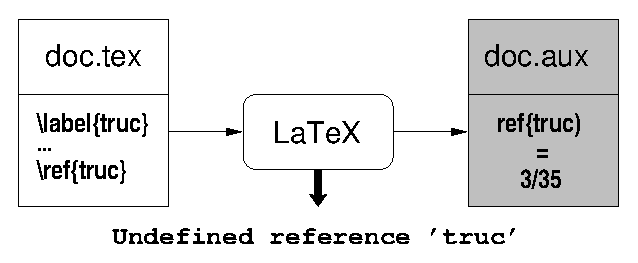
\includegraphics{img/ref1.eps}
    \end{center}
    \caption{使用\dm{.aux}的第一次编译}
    \label{fig:ref1}
  \end{figure}

  因此,此次编译时,会\LaTeX 发送警告,指出标记\dm{truc}未定义。
  \item 我们会进行第二次编译,这次编译会使用辅助文件的内容(如图\ref{fig:ref2}所示)。
  
  \begin{figure}[ht]
    \begin{center}
      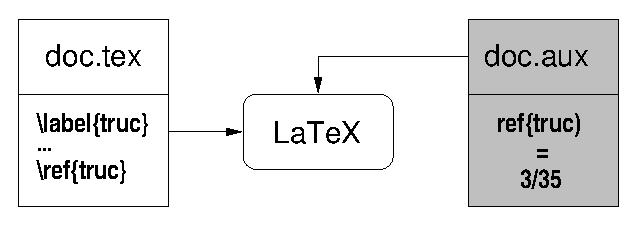
\includegraphics{img/ref2.eps}
    \end{center}
    \caption{使用\dm{.aux}的第二次编译}
    \label{fig:ref2}
  \end{figure}
\end{enumerate}

在以下情况中的引用定义是不正确的。

\begin{enumerate}
  \item 你插入了一个新的标记,并且在插入标记后第一次编译(引用\emph{未被定义})。此时,对于新插入的标记,会得到如下形式的消息:
  
  \begin{dmd}
  Reference 'vlunch' on page 2 undefined on input line 17.
  \end{dmd}

  \item 你在文档中引入的变化无疑会改变页码或对象(图片、方程等)的位置,因此引用会被\emph{错误定义}。在编译结束时,你会看到如下警告:
  
  \begin{dmd}
  Label(s) may have changed.\\
  Rerun to get cross-references right.
  \end{dmd}

  \item 你引用了一个不存在的标记。在这种情况下,再编译八百次也无济于事。
\end{enumerate}

\subsection{与目录的交互}

对于目录,你会发现,其原理与引用是类似的。在文档中插入指令\verb|\tableofcontents|意味着目录将会分两步创建,具体如下。

\begin{enumerate}
  \item 第一轮遍历会收集文档中与\emph{表题}相关的信息,并将其存入文件\codereplace{文件名}\dm{.toc}中(如图\ref{fig:toc1}所示)。
  
  \begin{figure}[ht]
    \begin{center}
      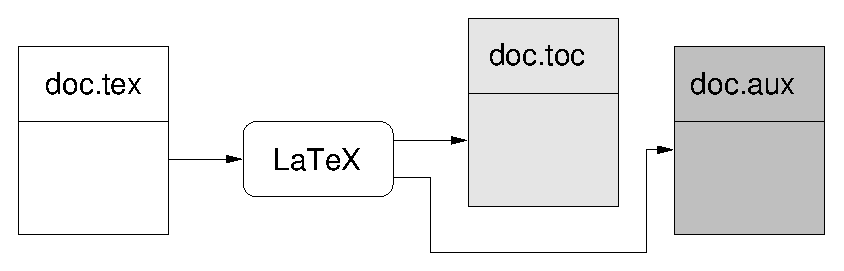
\includegraphics{img/toc1.eps}
    \end{center}
    \caption{使用\dm{.toc}的第一次编译}
    \label{fig:toc1}
  \end{figure}

  \item 第二轮遍历会使最终的文档中包含\codereplace{文件名}\dm{.toc},因此,目录也会被包含(如图\ref{fig:toc2}所示)。
  
  \begin{figure}[ht]
    \begin{center}
      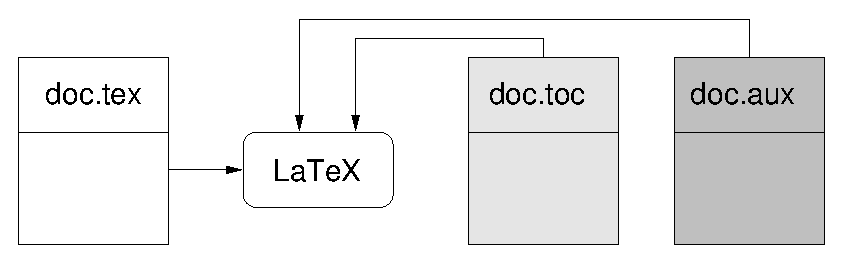
\includegraphics{img/toc2.eps}
    \end{center}
    \caption{使用\dm{.toc}的第二次编译}
    \label{fig:toc2}
  \end{figure}

\end{enumerate}

你可能会遇到这种情况:在写草稿时,文档已经包含了目录指令(\verb|tableofcontents|),而你又添加了新的章节指令。在这种情况下,新的章节只有经过\textbf{两次}编译后才会显示在目录中。

\subsection{一些建议}

要养成为每个文档生成目录的习惯。实际上,\LaTeX 会围绕你的\dm{.tex}文件生成多个文件\jz{
  这还没有涉及参考文献、索引、术语目录等。
}。另外,在起草文档时,不必过于关心目录是否时刻更新——它早晚会更新的!实际上,只有在\textbf{印刷}之前才有必要去确认所有的引用都是正确的。

最后,就像我们在不再能确定目标文件时会时不时运行一下\dm{make clean}指令一样,在看起来一切都运行不正常时,删掉辅助文件\celan{\S B.2}并重新编译是个好习惯。

\section{断字的处理}

\LaTeX 依靠\TeX 对特定的语言来实现不同的断字效果。这种算法在\TeX Book的附录H中有描述,也体现出\TeX 最成功的一面。通过检查文档打断段落的方式,可以识别出文档是不是由\LaTeX 生成的,因为其他很多软件都喜欢以在单词间添加更多空间的方式来处理此类问题。然而,也会有一些\LaTeX 无法正确断字的情况。在这种情况下,\LaTeX 会以以下两种“吓人的”信息之一为你给出警告:

\begin{dmd}
Underfull \backslash hbox (badness 1810) detected at line 33
\end{dmd}

或

\begin{dmd}
Overfull \backslash hbox (14.24376pt too wide) detected at line 41
\end{dmd}

\TeX 在很底层用你的文档生成一系列\emph{字盒}。每个字符都装入合适的字盒,字盒组合成词,再以类似的方式组合成行、成段,然后成页面。

这里以一种简单的方式总结和介绍原理。我们可以简单地理解为,\TeX 在水平模式下操纵\verb|\hbox|来组合单词,在竖直模式下操纵\verb|\vbox|来生成页面。此外,组合这些字盒时,\TeX 如果觉得结果不太美观,就会用以上述两种信息警告你。信息的含义如下。

\begin{itemize}
  \item \verb|Underfull \hbox|表示字盒组合得有些稀疏。通过显示badness的值,\TeX 会告诉你它认为当前行“有多丑”。如果一行文字排列得很完美,该值为0。在最差的情况下,该值为10000.
  \item \verb|Overfull \hbox|表示字盒有些太挤了。\TeX 可以以\dm{pt}为单位显示文字越界深入边缘的长度。
\end{itemize}

如果一个页面过于稀疏,\LaTeX 会以\verb|\vbox|代替\verb|\hbox|显示类似的消息。表\ref{tab:2.4}展示了同一句话的不同疏密程度\yz{
  表中的例句出自法国古典主义戏剧大师高乃依(Pierre Corneille)的戏剧《熙德》(\textit{Le Cid}),意为“哦,愤怒!哦,绝望!哦,宿敌!”。
}排列效果。

\newcommand{\phrase}[1]{\noindent\makebox[\width +
#1][s]{%
  Ô rage ! ô désespoir ! ô vieillesse ennemie !}\par}
\begin{table}[ht] 
\begin{center}
  % \addtolength{\extrarowheight}{4pt} 
  \begin{tabular}{|l|c|}
    \hline
    效果 & 评价 \\
    \hline
    % \typeout{UNDERFULL HBOX AUTORISE}%
    \phrase{1.0cm}  & 稀疏\\
    \phrase{0.75cm} & 稀疏\\
    \phrase{0.45cm} & 稀疏\\
    \hline
    % \typeout{UNDERFULL HBOX AUTORISE}%
    \phrase{0cm}    & 理想 \\ 
    \hline
    \phrase{-0.1cm} & 过密\\
    \phrase{-0.2cm} & 过密\\
    \phrase{-0.25cm} & 过密\\
    \hline
  \end{tabular}
  \caption{横向的不同疏密排列}
  \label{tab:2.4}
\end{center} 
\end{table}

\begin{ii}
  \makebox[\width+2pt][s]{可以在文档选项中启用\dm{draft},来使在出现\dm{Overfull \backslash hbox}问题的位置的侧栏显示一个黑色的\char"258C}
  方块,就像本段的侧栏一样。这个选项可以帮助快速定位导致问题的行。
\end{ii}

\subsection{控制断字}

对于以下情况,\LaTeX 的断字处理可能遇到困难。

\begin{itemize}
  \item 它不能识别需要打断的词——这是个极端情况。
  \item 不能打断的对象占据了需要打断的位置,例如\verb+\verb|...|+或方程类型的对象。
\end{itemize}

这里提供以下几个控制断字的方法。

\begin{exclamation}
如果以下方法都不能使你满意(如果你的句子中包含太多\TeX 不能打断的对象,就会产生这种情况),就只能想办法更换表达方式来规避问题了。
\end{exclamation}

\subsubsection{引导断字}

我们可以通过在必要的位置插入指令\verb|\-|来指出可以断字的位置,从而帮助\LaTeX 实现断字。例如,如果\LaTeX 不能成功地打断“nonmaiçavapamieu”\yz{
  作者的生造词,形似句子“Non, mais ça ne va pas mieux.”,意为“不,没有变得更好”。
}一词,我们可以输入:

\begin{dmd}
\verb|non\-mai\-ça\-va\-pa\-mieu|
\end{dmd}

如果这个词频繁出现,为了避免反复像上面这样给出指示,可以在文前部分输入指令\linebreak \verb|\hyphenation|:

\begin{dmd}
\verb|\hyphenation{non-mai-ça-va-pa-mieu}|
\end{dmd}

这样就可以告诉\LaTeX 这个生词的断字方式。

\subsubsection{强制断字}

通过输入指令\verb|\linebreak[|\codereplace{数字}\verb|]|,我们可以强制断字,但这样做可能带来灾难性的后果——如果你明白我的意思。参数\codereplace{数字}可以调节指令\verb|\linebreak|。你可以“腼腆”地给出指示——\verb|\linebreak[0]|,或是给出不容置疑的命令——\verb|\linebreak[4]|。

指令\verb|\pagebreak[|\codereplace{数字}\verb|]|可以打断页面。另一方面,还有两个指令可以用来换页:

\begin{itemize}
  \item \verb|\clearpage| 完成当前页面,换页另起。
  \item \verb|\cleardoublepage| 完成当前页面,并在双面模式下从奇数页另起。
\end{itemize}

这两条指令会强制\LaTeX 在布局过程中插入所有浮动的图像。%TODO 所以这句是在说啥???

\begin{ii}
另外一种对某些情况很实用的手动介入方式是将当前页面纵向长度加长,需要调用如下指令:

\begin{dmd}
  \backslash enlargethispage
\end{dmd}

指令需要给出尺寸,且其后需要插入一个空行:

\begin{tabbing}
  \verb|\enlargethispage{10cm}   | \= \leftarrow 针对过短的页面 \\
  ~\\
  \verb|[……一段过长的文字……]|\\
  \verb|\clearpage| \> \leftarrow 明确延长10 cm的页面的结尾
\end{tabbing}
\end{ii}

\subsubsection{防止断字}

有三种方式可以强制\LaTeX 不打断文本。

\begin{enumerate}
  \item 通过\verb|~|插入不可打断的空格。
  \item 通过\verb|\mbox{|\codereplace{单词}\verb|}|将词放入一个字盒中\jz{
    这是因为\TeX \textbf{永远不会}打断字盒。
  }。
  \item 对于防止换行使用指令\verb|\nolinebreak|:
  
  \begin{dmd}
  \backslash nolinebreak[\codereplace{数字}]
  \end{dmd}

  同样,为了防止换页,可以使用如下指令:

  \begin{dmd}
    \backslash nopagebreak[\codereplace{数字}]
  \end{dmd}

  其中\codereplace{数字}与\verb|\linebreak|或\verb|\pagebreak|中的作用一致。

\end{enumerate}

\section{小结}

本章介绍了\LaTeX 的标准功能。你如果专心地阅读至此,应该已经可以创建任何类型的简单文档了(目前还不能处理带有公式和图表的文档)。即使你还不能自由地定制你的文档,你的文档的排版质量也会足够好,不需要你提出很多形而上学的问题,如多大的页边距才“理想”、标题和文字间留出多少空白才“合适”……实际上,\LaTeX 中的默认特性已经足够满足全世界范围内有关印刷的大部分实用性规则。


\end{verbatim}
\verb+\backmatter +\textsl{\% 文档末尾的索引内容}
\begin{verbatim}
\bibliographstyle{plain} 
\bibliography{machin,bidule,truc}
\end{document}
\end{verbatim}
\end{dmd}

其中的指令\verb|\include|的作用在于,它们减少了你需要同时处理的章节数量,却依然保证了文档的完整性。为此,我们可以在文前部分使用指令\verb|\includeonly|:

\begin{dmd}
\verb|\includeonly{preface,savoir}|
\end{dmd}

使用该指令,可以仅编译前言部分(作为文件\dm{preface.tex}的内容)和文档\dm{savoir.tex}中的章节。

\begin{exclamation}
每条指令\verb|\include|都具有换页的效果,并且似乎没有规避该指令换页的方法。因此,你应该了解,\verb|\include|应当配合能够换页的章节指令(如\verb|\chapter|)使用。若要在插入其他文件时不换页,则应使用指令\verb|\input|,否则这种主文件机制就不会为你带来好处。
\end{exclamation}

最后需要注意到,\verb|\frontmatter|、\verb|\mainmatter|、\verb|\backmatter|这三条指令不是必需的。它们的作用是自动将页码改为罗马数字,常常用于介绍性质的文前页或其他短小部分(然而,它们只在文件类型\dm{book}中可用)。